\begin{figure}[ht]
\centering
% Thesis-wide categorical color palette
% Usage: % Thesis-wide categorical color palette
% Usage: % Thesis-wide categorical color palette
% Usage: \input{figures/palette} in any figure file
%
% Muted primary colors -- print-friendly, visually distinct.
% Inspired by Cooper Union's red/blue primaries, softened for
% academic figures. Use palA-palC for data series in scatter
% plots, line charts, bar charts, etc.

\definecolor{palA}{HTML}{1F77B4}   % Tableau blue
\definecolor{palB}{HTML}{D62728}   % Tableau red
\definecolor{palC}{HTML}{2CA02C}   % Tableau green
 in any figure file
%
% Muted primary colors -- print-friendly, visually distinct.
% Inspired by Cooper Union's red/blue primaries, softened for
% academic figures. Use palA-palC for data series in scatter
% plots, line charts, bar charts, etc.

\definecolor{palA}{HTML}{1F77B4}   % Tableau blue
\definecolor{palB}{HTML}{D62728}   % Tableau red
\definecolor{palC}{HTML}{2CA02C}   % Tableau green
 in any figure file
%
% Muted primary colors -- print-friendly, visually distinct.
% Inspired by Cooper Union's red/blue primaries, softened for
% academic figures. Use palA-palC for data series in scatter
% plots, line charts, bar charts, etc.

\definecolor{palA}{HTML}{1F77B4}   % Tableau blue
\definecolor{palB}{HTML}{D62728}   % Tableau red
\definecolor{palC}{HTML}{2CA02C}   % Tableau green

\definecolor{nodeblue}{HTML}{B8D2E6}
\definecolor{nodeborder}{HTML}{5A87B5}
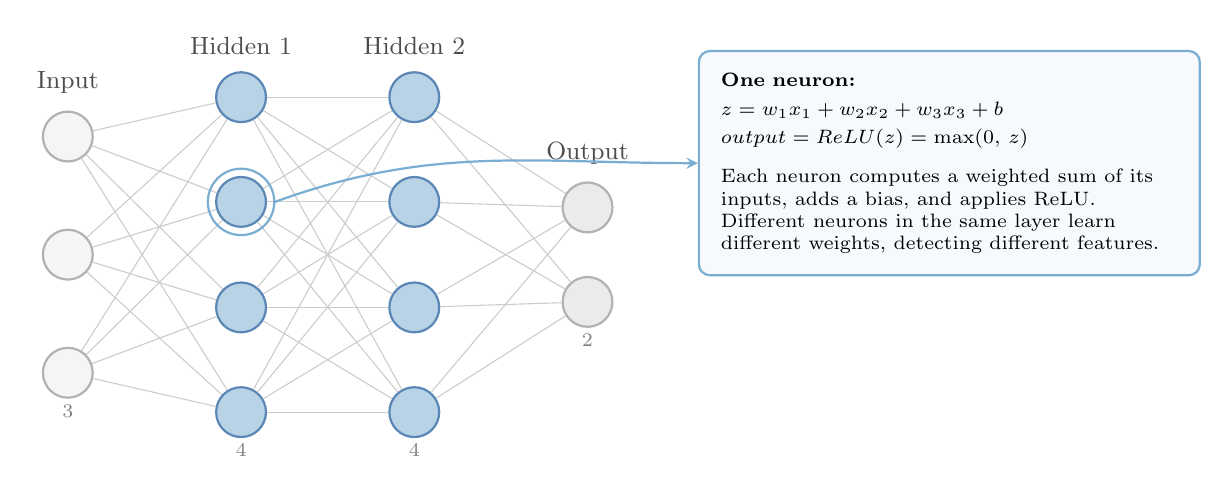
\begin{tikzpicture}[
    neuron/.style={circle, draw=nodeborder, thick, fill=nodeblue,
                   minimum size=18pt, inner sep=0pt},
    input/.style={circle, draw=black!30, thick, fill=black!4,
                  minimum size=18pt, inner sep=0pt},
    output/.style={circle, draw=black!30, thick, fill=black!8,
                   minimum size=18pt, inner sep=0pt},
    conn/.style={-, black!20},
    arr/.style={->, thick, >=stealth, black!40},
    lbl/.style={font=\small, text=black!70},
    sublbl/.style={font=\scriptsize, text=black!50},
    callout/.style={draw=palA!60, thick, rounded corners=4pt,
                    fill=palA!4},
]

% === Main network ===

% Layer x-positions
\def\xin{0}
\def\xha{2.2}
\def\xhb{4.4}
\def\xout{6.6}

% --- Input layer (3 nodes) ---
\foreach \i/\ypos in {1/1.5, 2/0, 3/-1.5} {
    \node[input] (i\i) at (\xin, \ypos) {};
}
\node[lbl, above=12pt] at (\xin, 1.5) {Input};
\node[sublbl, below=8pt] at (\xin, -1.5) {3};

% --- Hidden layer 1 (4 nodes) ---
\foreach \j/\ypos in {1/2.0, 2/0.67, 3/-0.67, 4/-2.0} {
    \node[neuron] (h1\j) at (\xha, \ypos) {};
}
\node[lbl, above=12pt] at (\xha, 2.0) {Hidden 1};
\node[sublbl, below=8pt] at (\xha, -2.0) {4};

% --- Hidden layer 2 (4 nodes) ---
\foreach \k/\ypos in {1/2.0, 2/0.67, 3/-0.67, 4/-2.0} {
    \node[neuron] (h2\k) at (\xhb, \ypos) {};
}
\node[lbl, above=12pt] at (\xhb, 2.0) {Hidden 2};
\node[sublbl, below=8pt] at (\xhb, -2.0) {4};

% --- Output layer (2 nodes) ---
\foreach \l/\ypos in {1/0.6, 2/-0.6} {
    \node[output] (o\l) at (\xout, \ypos) {};
}
\node[lbl, above=12pt] at (\xout, 0.6) {Output};
\node[sublbl, below=8pt] at (\xout, -0.6) {2};

% --- Connections ---
% Input -> Hidden 1
\foreach \i in {1,2,3} {
    \foreach \j in {1,2,3,4} {
        \draw[conn] (i\i) -- (h1\j);
    }
}
% Hidden 1 -> Hidden 2
\foreach \j in {1,2,3,4} {
    \foreach \k in {1,2,3,4} {
        \draw[conn] (h1\j) -- (h2\k);
    }
}
% Hidden 2 -> Output
\foreach \k in {1,2,3,4} {
    \foreach \l in {1,2} {
        \draw[conn] (h2\k) -- (o\l);
    }
}

% === Neuron callout ===
% Highlight neuron h1-2 (second from top in hidden layer 1)
\draw[palA!60, thick] (h12) circle (12pt);

% Callout box
\node[callout, anchor=north west, text width=5.8cm,
      inner sep=8pt, font=\scriptsize]
    (callbox) at (8.0, 2.6) {%
    \textbf{One neuron:}\\[4pt]
    \begin{tabular}{@{}l@{}}
    $z = w_1 x_1 + w_2 x_2 + w_3 x_3 + b$ \\[2pt]
    $\text{output} = \text{ReLU}(z) = \max(0,\, z)$
    \end{tabular}\\[6pt]
    Each neuron computes a weighted sum of its\\
    inputs, adds a bias, and applies ReLU.\\
    Different neurons in the same layer learn\\
    different weights, detecting different features.
};

% Arrow from highlighted neuron to callout
\draw[arr, palA!60] (h12.east) ++(0.1, 0)
    to[out=20, in=180] (callbox.west);

\end{tikzpicture}
\caption{A feed-forward neural network with three input nodes, two
  hidden layers of four neurons each, and two output nodes. Every
  neuron in one layer connects to every neuron in the next (fully
  connected). The callout shows the computation inside a single
  neuron.}
\label{fig:feedforward-network}
\end{figure}
